\documentclass[12pt,letter]{article}\usepackage[]{graphicx}\usepackage[]{color}
% maxwidth is the original width if it is less than linewidth
% otherwise use linewidth (to make sure the graphics do not exceed the margin)
\makeatletter
\def\maxwidth{ %
  \ifdim\Gin@nat@width>\linewidth
    \linewidth
  \else
    \Gin@nat@width
  \fi
}
\makeatother

\definecolor{fgcolor}{rgb}{0.345, 0.345, 0.345}
\newcommand{\hlnum}[1]{\textcolor[rgb]{0.686,0.059,0.569}{#1}}%
\newcommand{\hlstr}[1]{\textcolor[rgb]{0.192,0.494,0.8}{#1}}%
\newcommand{\hlcom}[1]{\textcolor[rgb]{0.678,0.584,0.686}{\textit{#1}}}%
\newcommand{\hlopt}[1]{\textcolor[rgb]{0,0,0}{#1}}%
\newcommand{\hlstd}[1]{\textcolor[rgb]{0.345,0.345,0.345}{#1}}%
\newcommand{\hlkwa}[1]{\textcolor[rgb]{0.161,0.373,0.58}{\textbf{#1}}}%
\newcommand{\hlkwb}[1]{\textcolor[rgb]{0.69,0.353,0.396}{#1}}%
\newcommand{\hlkwc}[1]{\textcolor[rgb]{0.333,0.667,0.333}{#1}}%
\newcommand{\hlkwd}[1]{\textcolor[rgb]{0.737,0.353,0.396}{\textbf{#1}}}%
\let\hlipl\hlkwb

\usepackage{framed}
\makeatletter
\newenvironment{kframe}{%
 \def\at@end@of@kframe{}%
 \ifinner\ifhmode%
  \def\at@end@of@kframe{\end{minipage}}%
  \begin{minipage}{\columnwidth}%
 \fi\fi%
 \def\FrameCommand##1{\hskip\@totalleftmargin \hskip-\fboxsep
 \colorbox{shadecolor}{##1}\hskip-\fboxsep
     % There is no \\@totalrightmargin, so:
     \hskip-\linewidth \hskip-\@totalleftmargin \hskip\columnwidth}%
 \MakeFramed {\advance\hsize-\width
   \@totalleftmargin\z@ \linewidth\hsize
   \@setminipage}}%
 {\par\unskip\endMakeFramed%
 \at@end@of@kframe}
\makeatother

\definecolor{shadecolor}{rgb}{.97, .97, .97}
\definecolor{messagecolor}{rgb}{0, 0, 0}
\definecolor{warningcolor}{rgb}{1, 0, 1}
\definecolor{errorcolor}{rgb}{1, 0, 0}
\newenvironment{knitrout}{}{} % an empty environment to be redefined in TeX

\usepackage{alltt}

%########################################################################################
%            						PACKAGES
%########################################################################################

\usepackage{authblk} % for author affiliations
\usepackage{float} % for H in figures and tables
\usepackage{amsmath,amsthm,amssymb,bbm,mathrsfs,mathtools,xfrac} %math stuff
%\usepackage{cleveref}
%\newcommand{\crefrangeconjunction}{--}

\usepackage[sort]{natbib}   % bibliography omit 'round' option if you prefer square brackets
\usepackage{placeins} % for \FloatBarrier
\usepackage[pagebackref=true,bookmarks]{hyperref}
\hypersetup{
	unicode=false,
	pdftoolbar=true,
	pdfmenubar=true,
	pdffitwindow=false,     % window fit to page when opened
	pdfstartview={FitH},    % fits the width of the page to the window
	pdftitle={Sparse Additive Interaction Learning},    % title
	pdfauthor={Sahir Rai Bhatnagar},     % author
	pdfsubject={sail manuscript},   % subject of the document
	pdfcreator={Sahir Rai Bhatnagar},   % creator of the document
	pdfproducer={Sahir Rai Bhatnagar}, % producer of the document
	pdfkeywords={}, % list of keywords
	pdfnewwindow=true,      % links in new window
	colorlinks=true,       % false: boxed links; true: colored links
	linkcolor=red,          % color of internal links (change box color with linkbordercolor)
	citecolor=blue,        % color of links to bibliography
	filecolor=black,      % color of file links
	urlcolor=cyan           % color of external links
}
\usepackage[utf8]{inputenc} % for french accents
\usepackage[T1]{fontenc} % for french accents
\usepackage{ctable} % load after tikz. used for tables
\usepackage{pifont}% http://ctan.org/pkg/pifont
\newcommand{\cmark}{\ding{51}}%
\newcommand{\xmark}{\ding{55}}%
\def\widebar#1{\overline{#1}}
\usepackage{array}
\newcolumntype{L}{>{\centering\arraybackslash}m{3cm}} % used for text wrapping in ctable
\usepackage{color, colortbl, xcolor, comment}
\usepackage{subfig}
\usepackage{tcolorbox} % for box around text
%\usepackage[ruled,vlined,linesnumbered,noresetcount]{algorithm2e}
%\usepackage[ruled,vlined,noresetcount]{algorithm2e}
\usepackage{algorithm}
\usepackage{chngcntr} % for figure labels in appendix
%\usepackage[ruled,vlined,noresetcount]{algorithm2e}
\usepackage[noend]{algpseudocode}
\algrenewcommand\textproc{}% Used to be \textsc
\algdef{SE}[SUBALG]{Indent}{EndIndent}{}{\algorithmicend\ }%
\algtext*{Indent}
\algtext*{EndIndent}
%\usepackage[american]{babel}
%\let\tnote\relax

%\usepackage{csquotes}



%\usepackage[style=apa,sortcites=true,sorting=nyt,backend=biber]{biblatex}
%\usepackage{epstopdf}

%\usepackage{tabulary}
%\usepackage{siunitx}
%\sisetup{output-exponent-marker=\ensuremath{\mathrm{e}}}
%\AtBeginEnvironment{tabulary}{\onehalfspacing}
%\usepackage{multirow}
%\usepackage{ctable} % NEED TO LOAD CTABLE AFTER TIKZ FOR SOME REASON
%\usepackage{array}
%\newcolumntype{L}{>{\centering\arraybackslash}m{3cm}} % used for text wrapping in ctable
%\usepackage{enumitem}
% These packages are all incorporated in the memoir class to one degree or another...


%########################################################################################
%            						CUSTOM COMMANDS
%########################################################################################

\newtheorem{theorem}{Theorem}
\newtheorem{proposition}{Proposition}
\newtheorem{lemma}{Lemma}

\newcommand{\sgn}{\operatorname{sgn}}
\newcommand{\Op}{O_{P}}
\newcommand{\op}{o_{P}}
\newcommand{\ddd}{,\ldots,}
%\global\long\def\ddd{,\ldots,}
\newcommand{\sail}{\texttt{sail}}
\newcommand{\tm}[1]{\textrm{{#1}}}
\newcommand{\bx}{\textbf{\emph{x}}}
\newcommand{\by}{\textbf{\emph{y}}}
\newcommand{\bX}{\textbf{\emph{X}}}
\newcommand{\bW}{\textbf{\emph{W}}}
\newcommand{\bY}{\textbf{\emph{Y}}}
\newcommand{\bD}{\textbf{\text{D}}}
\newcommand{\bXtilde}{\widetilde{\bX}}
\newcommand{\bYtilde}{\widetilde{\bY}}
\newcommand{\bDtilde}{\widetilde{\bD}}
\newcommand{\Xtilde}{\widetilde{X}}
\newcommand{\Ytilde}{\widetilde{Y}}
\newcommand{\Dtilde}{\widetilde{D}}
\newcommand{\bu}{\textbf{u}}
\newcommand{\bU}{\textbf{\emph{U}}}
\newcommand{\bV}{\textbf{\emph{V}}}
\newcommand{\bE}{\textbf{\emph{E}}}
\newcommand{\bb}{\textbf{\emph{b}}}
\newcommand{\bI}{\textbf{\emph{I}}}
\newcommand{\be}{\boldsymbol{\varepsilon}}
\newcommand{\bSigma}{\boldsymbol{\Sigma}}
\newcommand{\bLambda}{\boldsymbol{\Lambda}}
\newcommand{\bTheta}{\boldsymbol{\Theta}}
\newcommand{\balpha}{\boldsymbol{\alpha}}
\newcommand{\btau}{\boldsymbol{\tau}}
\newcommand{\bgamma}{\boldsymbol{\gamma}}
%\newcommand{\ltwonorm}[1]{\lVert #1 \rVert}
\newcommand{\mb}[1]{\mathbf{#1}}
\newcommand{\mc}[2]{\multicolumn{#1}{c}{#2}}
\newcommand{\mcl}[2]{\multicolumn{#1}{l}{#2}}
\definecolor{Gray}{gray}{0.9}
\newcommand {\bs}{\boldsymbol}
%\newcommand{\norm}[1]{\left\Vert #1 \right\Vert}
\newcommand{\xf}{\mathcal{X}}
\newcommand{\pfrac}[2]{\left( \frac{#1}{#2}\right)}
\newcommand{\e}{{\mathsf E}}
\newcommand{\bt}{\boldsymbol{\theta}}
\newcommand{\bmu}{\boldsymbol{\mu}}
\newcommand{\bbeta}{\boldsymbol{\beta}}
\newcommand{\btheta}{\boldsymbol{\theta}}
\newcommand{\bPhi}{\boldsymbol{\Phi}}
\newcommand{\bPsi}{\boldsymbol{\Psi}}
\DeclareMathOperator*{\argmin}{arg\,min}
\DeclareMathOperator*{\argmax}{arg\,max}
\DeclareMathOperator{\diag}{diag} % operator and subscript

\DeclarePairedDelimiter\abs{\lvert}{\rvert}%
\DeclarePairedDelimiter\norm{\lVert}{\rVert}%

\global\long\def\ddd{,\ldots,}


\newcommand{\bthetastar}{\boldsymbol{\theta}^{*}}
\newcommand{\bThetastar}{\boldsymbol{\Theta}^{*}}
\newcommand{\bdelta}{\boldsymbol{\delta}}
\newcommand{\A}{\mathcal{A}}
\newcommand{\mH}{\mathcal{H}}

% Swap the definition of \abs* and \norm*, so that \abs
% and \norm resizes the size of the brackets, and the
% starred version does not.
\makeatletter
\let\oldabs\abs
\def\abs{\@ifstar{\oldabs}{\oldabs*}}
%
\let\oldnorm\norm
\def\norm{\@ifstar{\oldnorm}{\oldnorm*}}
\makeatother

%########################################################################################
%            						FANCY HEADER STUFF
%########################################################################################
\usepackage{lastpage}
\usepackage{fancyhdr}
\cfoot{\thepage}
\lhead[\leftmark]{}
\rhead[]{\leftmark}
\makeatletter
\makeatother
%\lfoot{} \cfoot{ } \rfoot{{\small{\em Page \thepage \ of \pageref{LastPage}}}}
\lfoot{} \cfoot{ } \rfoot{{\small{\em Page \thepage}}}

%########################################################################################
%            						SPACING
%########################################################################################

\usepackage[parfill]{parskip} % Activate to begin paragraphs with an empty line rather than an indent
%\usepackage[left=.1in,right=.1in,top=.1in,bottom=.1in]{geometry}
\usepackage[margin=1in]{geometry}
\usepackage{setspace}
\doublespacing

%########################################################################################
%            						TITLE and AUTHORS
%########################################################################################

\title{A Sparse Additive Model for High-Dimensional Interactions with an Exposure Variable}
%\author{SRB}

%David L Olds Department of Pediatrics, University of Colorado School of Medicine, Denver David.Olds@ucdenver.edu

%Michael S. Kobor Department of Medical Genetics, University of British Columbia msk@cmmt.ubc.ca

%Michael J. Meaney, Singapore Institute for Clinical Sciences, Singapore; McGill University, michael.meaney@mcgill.ca

\author[1,2]{Sahir R Bhatnagar}
\author[3,4]{Tianyuan Lu}
\author[5]{Amanda Lovato}
\author[6]{David L Olds}
\author[7]{Michael S Kobor}
\author[8]{Michael J Meaney}
\author[9]{Kieran O'Donnell}
\author[10]{Yi Yang}
\author[1,3,5]{\mbox{Celia MT Greenwood}}

\affil[1]{Department of Epidemiology, Biostatistics and Occupational Health, McGill University}
\affil[2]{Department of Diagnostic Radiology, McGill University}
\affil[3]{Quantitative Life Sciences, McGill University}
\affil[4]{Lady Davis Institute, Jewish General Hospital, Montr\'{e}al, QC}
\affil[5]{Statistics Canada, Ottawa, ON}
\affil[6]{Department of Pediatrics, University of Colorado School of Medicine, Denver}
\affil[7]{Department of Medical Genetics, University of British Columbia, BC}
\affil[8]{Singapore Institute for Clinical Sciences, Singapore; McGill University}
\affil[9]{Department of Psychiatry, McGill University}
\affil[10]{Department of Mathematics and Statistics, McGill University}
\affil[11]{Departments of Oncology and Human Genetics, McGill University}

%\date{October 19, 2019}

%########################################################################################
%            						START OF DOCUMENT
%########################################################################################
% NOTE: To produce blinded version, replace "1" with "0" below.
\newcommand{\blind}{1}

\usepackage{lineno}
\linenumbers


\let\oldbibliography\thebibliography
\renewcommand{\thebibliography}[1]{\oldbibliography{#1}
	\setlength{\itemsep}{0pt}} %Reducing spacing in the bibliography.
\IfFileExists{upquote.sty}{\usepackage{upquote}}{}
\begin{document}







\if1\blind
{
	\maketitle
} \fi

\if0\blind
{
	\bigskip
	\bigskip
	\bigskip
	\begin{center}
		{\LARGE\bf A Sparse Additive Model for High-Dimensional Interactions with an Exposure Variable}
	\end{center}
	\medskip
} \fi

\bigskip


\pagestyle{fancy}









\begin{knitrout}\scriptsize
\definecolor{shadecolor}{rgb}{0.969, 0.969, 0.969}\color{fgcolor}\begin{kframe}
\begin{verbatim}
## /scratch/bhatnagar-lab/sbhatnagar/git_repositories/sail/manuscript/bin
## +-- ADNI.R
## +-- PRS_bootstrap.R
## +-- PRS_eval_functions.R
## +-- PRS_method_functions.R
## +-- PRS_model_functions.R
## +-- PRS_plot_functions.R
## +-- PRS_plots.R
## +-- README_for_CSDA_Figures.Rnw
## +-- README_for_CSDA_Figures.pdf
## +-- README_for_CSDA_Figures.tex
## +-- cache
## |   +-- __packages
## |   +-- globals_6d1d04419b10b1a06759621e8a2eb8a6.RData
## |   +-- globals_6d1d04419b10b1a06759621e8a2eb8a6.rdb
## |   +-- globals_6d1d04419b10b1a06759621e8a2eb8a6.rdx
## |   +-- packages_9258a6f76ff684c0e2fd1b9c0ebacc65.RData
## |   +-- packages_9258a6f76ff684c0e2fd1b9c0ebacc65.rdb
## |   +-- packages_9258a6f76ff684c0e2fd1b9c0ebacc65.rdx
## |   +-- plot-mse-sim_9c0c9a1ddefc6e0131421d7b889a78cc.RData
## |   +-- plot-mse-sim_9c0c9a1ddefc6e0131421d7b889a78cc.rdb
## |   +-- plot-mse-sim_9c0c9a1ddefc6e0131421d7b889a78cc.rdx
## |   +-- setup2_900cd6b26f4a65ef22443e3819f71205.RData
## |   +-- setup2_900cd6b26f4a65ef22443e3819f71205.rdb
## |   +-- setup2_900cd6b26f4a65ef22443e3819f71205.rdx
## |   +-- simulation-results_05ea566347202b9db8e06fd8152aac10.RData
## |   +-- simulation-results_05ea566347202b9db8e06fd8152aac10.rdb
## |   +-- simulation-results_05ea566347202b9db8e06fd8152aac10.rdx
## |   +-- toy-effects_601ac4af2c99af20848947802c3de27d.RData
## |   +-- toy-effects_601ac4af2c99af20848947802c3de27d.rdb
## |   +-- toy-effects_601ac4af2c99af20848947802c3de27d.rdx
## |   +-- toy-example_a90f8c38d0355dd05704afeb06d0c2c6.RData
## |   +-- toy-example_a90f8c38d0355dd05704afeb06d0c2c6.rdb
## |   +-- toy-example_a90f8c38d0355dd05704afeb06d0c2c6.rdx
## |   +-- toy-solution-path_991c1813a5d6d78869c629849579836d.RData
## |   +-- toy-solution-path_991c1813a5d6d78869c629849579836d.rdb
## |   +-- toy-solution-path_991c1813a5d6d78869c629849579836d.rdx
## |   +-- unnamed-chunk-1_9950a44ce550dc548513d2b840367e35.RData
## |   +-- unnamed-chunk-1_9950a44ce550dc548513d2b840367e35.rdb
## |   \-- unnamed-chunk-1_9950a44ce550dc548513d2b840367e35.rdx
## +-- figure
## |   +-- plot-mse-sim-1.pdf
## |   +-- toy-effects-1.pdf
## |   \-- toy-solution-path-1.pdf
## +-- intro.R
## +-- setup.R
## +-- simulation.R
## +-- support_bootstrap.R
## \-- support_plots.R
\end{verbatim}
\end{kframe}
\end{knitrout}


\section{Figure 1 - Toy example solution path and effects}




\begin{knitrout}\scriptsize
\definecolor{shadecolor}{rgb}{0.969, 0.969, 0.969}\color{fgcolor}\begin{figure}[H]

{\centering 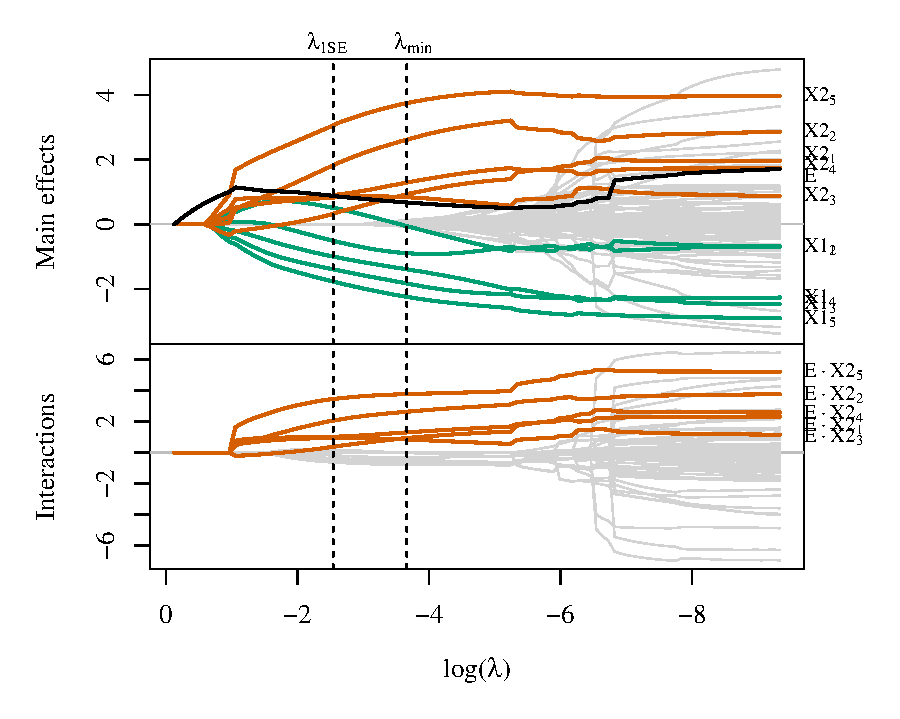
\includegraphics[width=1\linewidth]{figure/toy-solution-path-1} 

}

\caption[Toy example solution path for main effects (top) and interactions (bottom)]{Toy example solution path for main effects (top) and interactions (bottom). $\left\lbrace X1_1, X1_2, X1_3 \right\rbrace$ and $\left\lbrace X2_1, X2_2, X2_3 \right\rbrace$ are the three basis coefficients for $X_1$ and $X_2$, respectively. $\lambda_{1SE}$ is the largest value of penalization for which the CV error is within one standard error of the minimizing value $\lambda_{min}$.}\label{fig:toy-solution-path}
\end{figure}

\end{knitrout}

In Figure~\ref{fig:toy-effects}, we plot the true and estimated component functions $\hat{f}_1(X_1)$ and $E \cdot \hat{f}_2(X_2)$, and their estimates from this analysis with \texttt{sail}.
We are able to capture the shape of the correct functional form, but the means are not well aligned with the data. Lack-of-fit for $f_1(X_1)$ can be partially explained by acknowledging that \sail ~is trying to fit a cubic spline to a linear function.
Nevertheless, this example demonstrates that \sail ~can still identify trends reasonably well.

\begin{knitrout}\scriptsize
\definecolor{shadecolor}{rgb}{0.969, 0.969, 0.969}\color{fgcolor}\begin{figure}[H]

{\centering 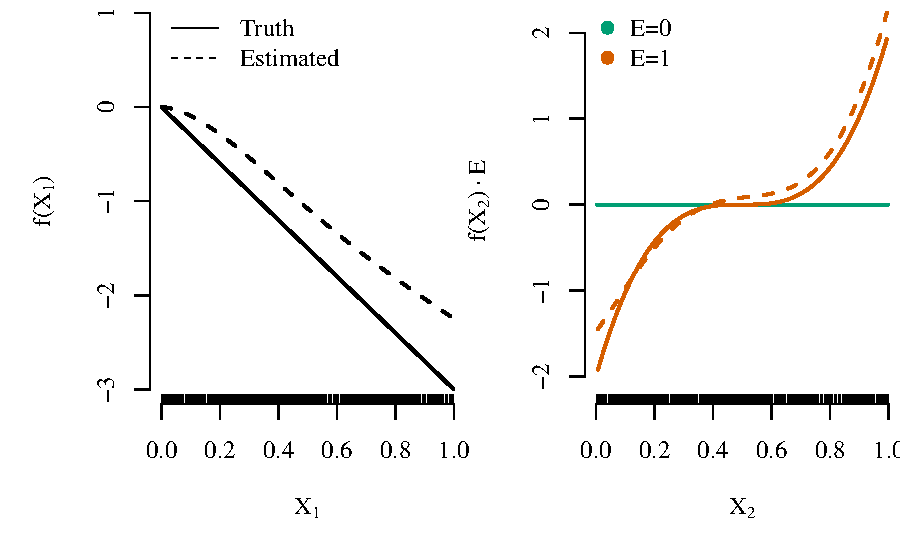
\includegraphics[width=1\linewidth]{figure/toy-effects-1} 

}

\caption[Estimated smooth functions for $X_1$ and the $X_2 \cdot E$ interaction by the \texttt{sail} method based on $\lambda_{min}$]{Estimated smooth functions for $X_1$ and the $X_2 \cdot E$ interaction by the \texttt{sail} method based on $\lambda_{min}$.}\label{fig:toy-effects}
\end{figure}

\end{knitrout}



\section{Figure 2 - Test set MSE}


\begin{knitrout}\scriptsize
\definecolor{shadecolor}{rgb}{0.969, 0.969, 0.969}\color{fgcolor}\begin{kframe}


{\ttfamily\noindent\bfseries\color{errorcolor}{\#\# Error in `:=`(scenario, as.numeric(as.character(stringr::str\_extract\_all(parameterIndex, : Check that is.data.table(DT) == TRUE. Otherwise, := and `:=`(...) are defined for use in j, once only and in particular ways. See help("{}:="{}).}}

{\ttfamily\noindent\bfseries\color{errorcolor}{\#\# Error in `:=`(scen, ifelse(scenario == 1, "{}Strong Hierarchy"{}, ifelse(scenario == : Check that is.data.table(DT) == TRUE. Otherwise, := and `:=`(...) are defined for use in j, once only and in particular ways. See help("{}:="{}).}}

{\ttfamily\noindent\bfseries\color{errorcolor}{\#\# Error in `:=`(scen, factor(scen, levels = c("{}Strong Hierarchy"{}, "{}Weak Hierarchy"{}, : Check that is.data.table(DT) == TRUE. Otherwise, := and `:=`(...) are defined for use in j, once only and in particular ways. See help("{}:="{}).}}\end{kframe}
\end{knitrout}


\begin{knitrout}\scriptsize
\definecolor{shadecolor}{rgb}{0.969, 0.969, 0.969}\color{fgcolor}\begin{figure}[h]

{\centering 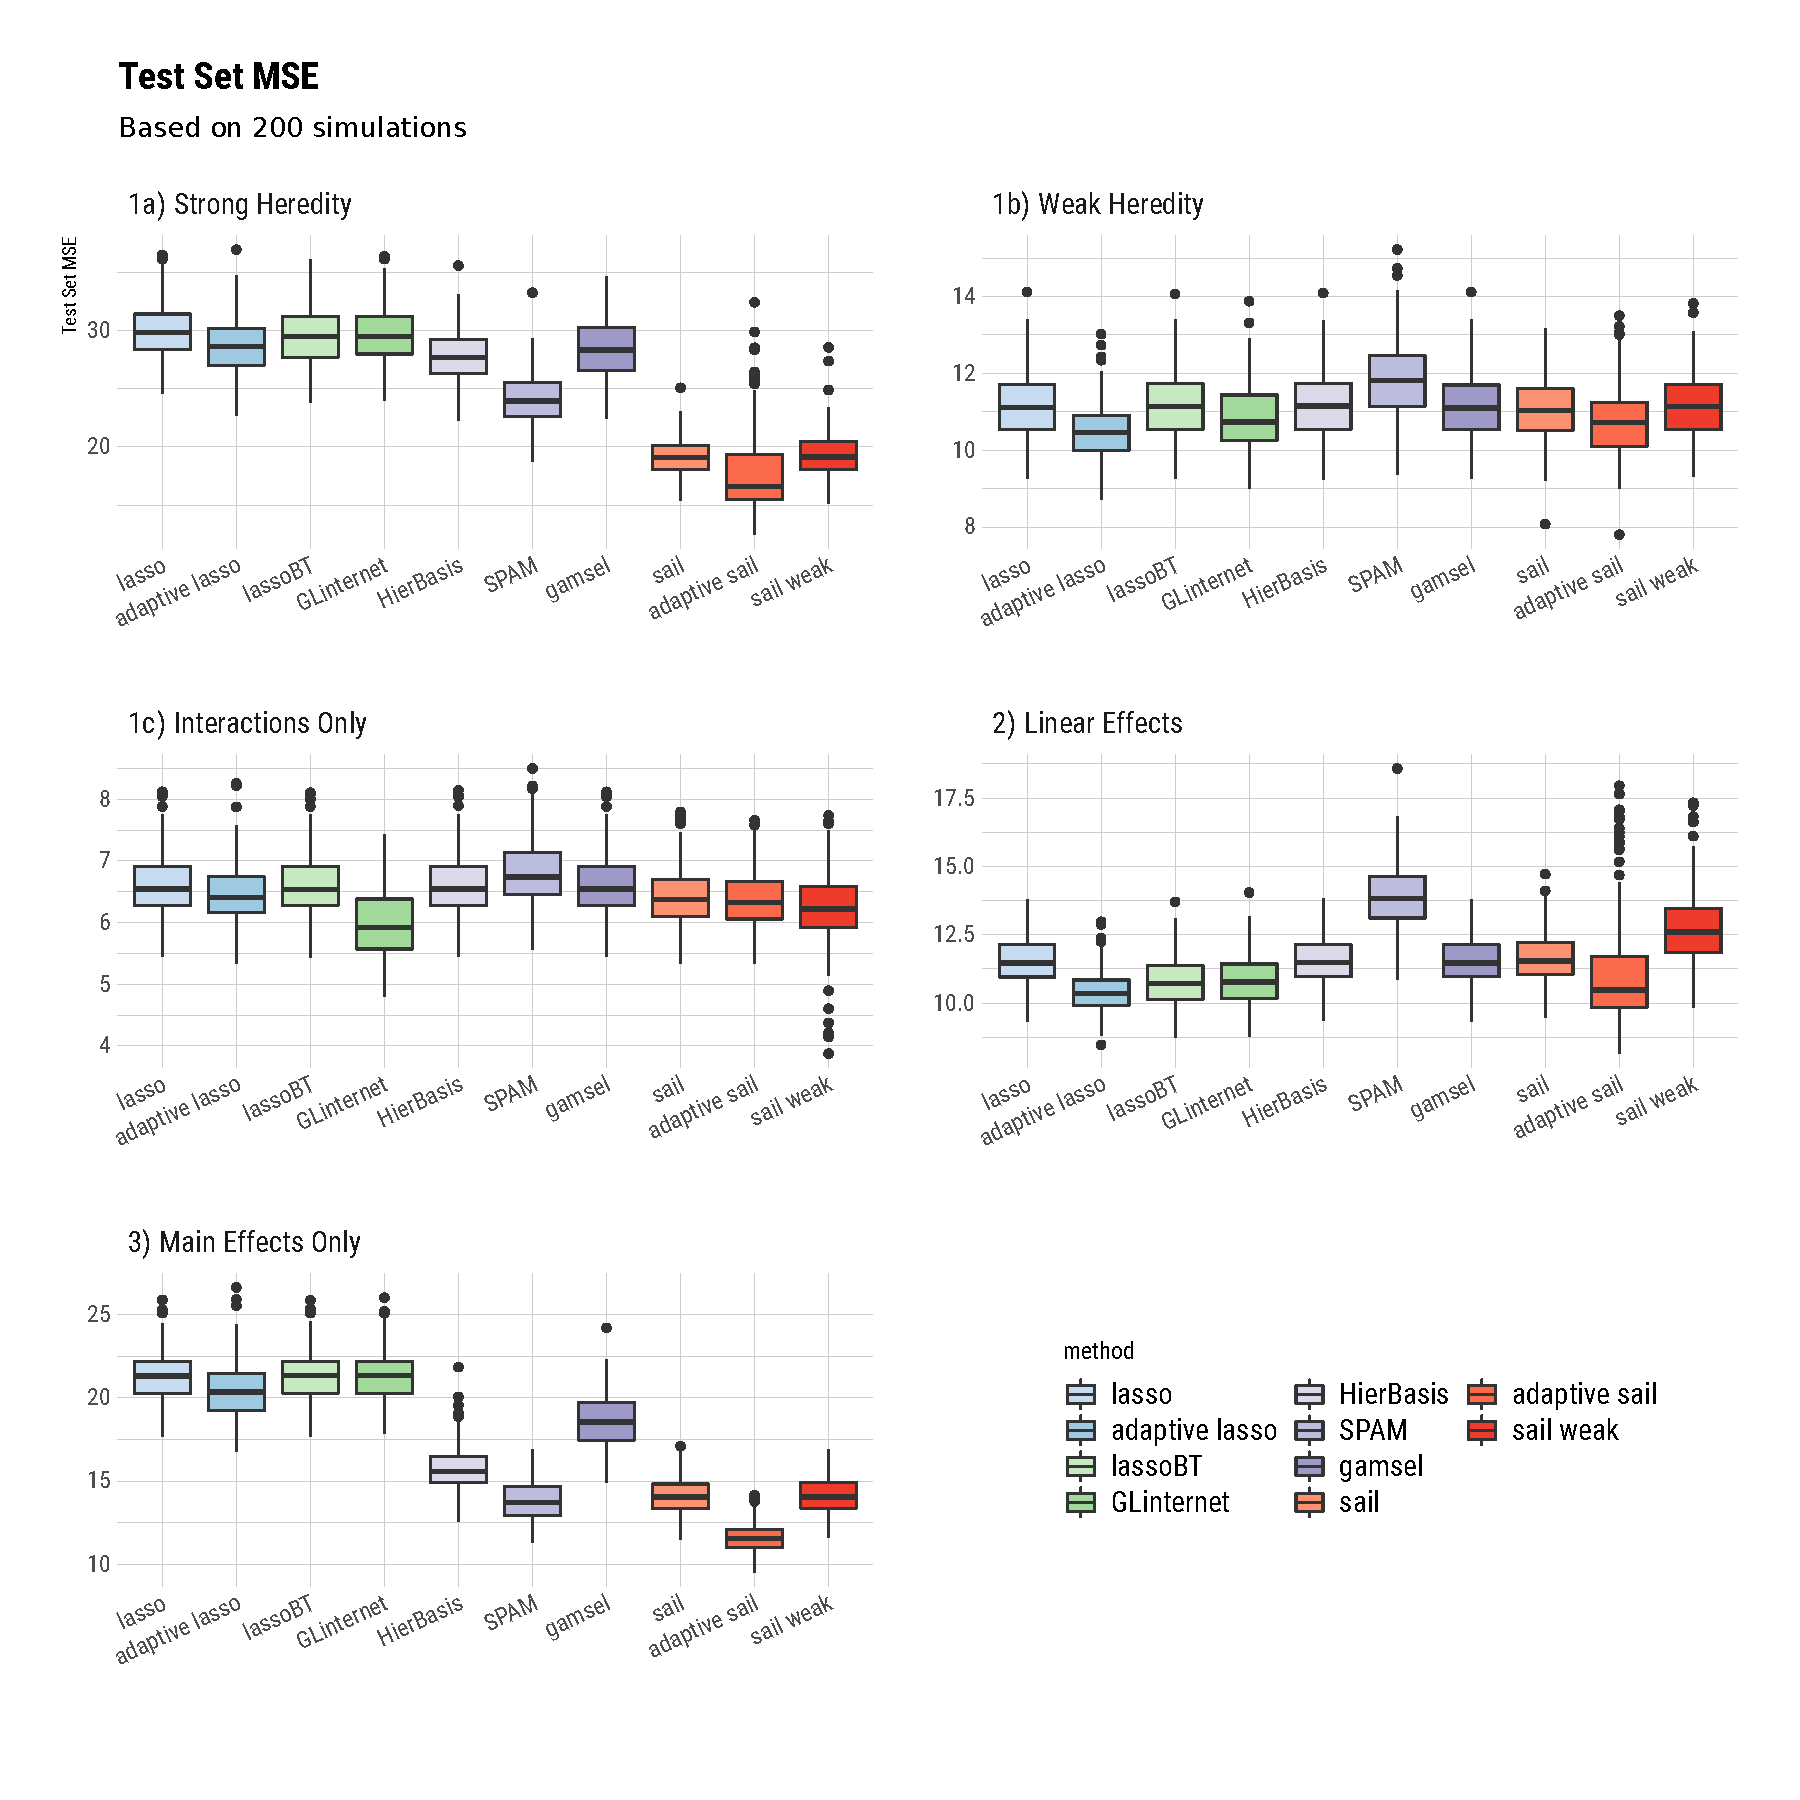
\includegraphics[width=1\linewidth]{figure/plot-mse-sim-1} 

}

\caption[Boxplots of the test set mean squared error from 200 simulations for each of the five simulation scenarios]{Boxplots of the test set mean squared error from 200 simulations for each of the five simulation scenarios.}\label{fig:plot-mse-sim}
\end{figure}

\end{knitrout}



\section{Table 1}






  %%%%%%%%%%%%%%%%%%%%%%%%%%%%%%%%%%%%%%%%%%%%%%%%%%%%%%%%%%%%%%%%%%%%%%%%%%%%%%%%%%%%%
%
%                                     TABLE 2
%
%
%%%%%%%%%%%%%%%%%%%%%%%%%%%%%%%%%%%%%%%%%%%%%%%%%%%%%%%%%%%%%%%%%%%%%%%%%%%%%%%%%%%%%

% latex table generated in R 4.0.3 by xtable 1.8-4 package
% Sun Sep  5 22:14:11 2021
%\multicolumn{#1}{c}{#2}
% see simulation.R pasted the xtable output here

%\begin{landscape}
\begin{sidewaystable}
%\begin{table}
\small
	\centering
	\caption{Mean (standard deviation) of the number of selected variables ($|\widehat{\mathcal{J}}|$), true positive rate (TPR) and false positive rate (FPR) as a percentage from 200 simulations for each of the five scenarios. $|\mathcal{J}|$ is the number of truly associated variables.}
	\label{tab:resultmultinom}
	\begin{tabular}{lcccccccccccccc}
		\hline
		&  \mc{2}{Linear}       &  &  \mc{2}{Linear}        & &  \mc{3}{Non-linear}   & & \mc{3}{Non-linear}  \\
&  \mc{2}{Main Effects}  &  &  \mc{2}{Interactions} & &  \mc{3}{Main Effects} & & \mc{3}{Interactions}  \\
\cmidrule{2-3}\cmidrule{5-6}\cmidrule{8-10}\cmidrule{12-14} % Important: no space before \cmidrule
& lasso &  adaptive  & & lassoBT   & GLinternet & & HierBasis  & SPAM  & gamsel & & sail &  adaptive  & sail  \\
&      &  lasso     & &    &  & &   &   &  & &  &  sail  & weak \\
\hline
\mcl{3}{1a) Strong heredity ($|\mathcal{J}|=7$)}   \\
$|\widehat{\mathcal{J}}|$ & 28 (15) & 8 (4) & & 35 (18) & 40 (20)  & & 133 (48) & 42 (19) & 46 (21) & &  21 (3) & 8 (3) & 21 (3) \\
TPR                        & 53.9 (8.4) & 49.3 (10.1) &  & 61.7 (11.5) & 66.4 (14.0)  & & 65.2 (8.1) & 60.9 (8.5) & 56.9 (7.7)  & & 86.8 (8.0) & 81.4 (13.0) & 82.1 (10.9) \\
FPR                        & 1.2 (0.7) & 0.2 (0.2)  & & 1.5 (0.9) & 1.8 (1.0)  & & 6.5 (2.4) & 1.9 (0.9) & 2.1 (1.1)  & & 0.8 (0.1) & 0.1 (0.1) & 0.8 (0.1) \ML
\mcl{3}{1b) Weak heredity ($|\mathcal{J}|=5$)} \\
$|\widehat{\mathcal{J}}|$ & 19 (12) & 4 (2)  & & 20 (13) & 38 (23) &  & 24 (23) & 28 (16) & 21 (15)  & & 16 (7) & 5 (3) & 14 (10) \\
TPR & 40.7 (3.6) & 40.1 (1.4)  & & 40.8 (3.8) & 64.1 (14.9)  & & 42.2 (6.3) & 53.9 (9.4) & 42.7 (6.8) & &  50.5 (10.4) & 46.4 (10.1) & 55.0 (13.7) \\
FPR & 0.9 (0.6) & 0.1 (0.1)  & & 0.9 (0.7) & 1.7 (1.1)  & & 1.1 (1.1) & 1.2 (0.8) & 1.0 (0.7)  & & 0.7 (0.3) & 0.2 (0.1) & 0.6 (0.5) \\
\hline
\mcl{3}{1c) Interactions Only ($|\mathcal{J}|=2$)}\\
$|\widehat{\mathcal{J}}|$ & 12 (12) & 3 (2)  & & 14 (13) & 38 (21)  & & 12 (13) & 13 (12) & 12 (12)  & & 7 (7) & 2 (2) & 26 (30) \\
TPR & 0.0 (0.0) & 0.0 (0.0)  & & 0.0 (0.0) & 81.4 (27.0)  & & 0.0 (0.0) & 0.0 (0.0) & 0.0 (0.0)  & & 0.0 (0.0) & 0.0 (0.0) & 22.9 (36.9) \\
FPR & 0.6 (0.6) & 0.6 (6.9)  & & 0.7 (0.7) & 1.8 (1.0)  & & 0.6 (0.7) & 0.7 (0.6) & 0.6 (0.6)  & & 0.4 (0.3) & 0.1 (0.1) & 1.3 (1.5) \\
\hline
\mcl{3}{2) Linear Effects ($|\mathcal{J}|=7$)}\\
$|\widehat{\mathcal{J}}|$ & 37 (17) & 8 (3)  & & 48 (19) & 51 (23)  & & 37 (19) & 42 (19) & 37 (16)  & & 20 (4) & 11 (4) & 20 (4) \\
TPR & 70.4 (3.7) & 67.2 (6.7)  & & 72.3 (6.3) & 93.4 (8.5) &  & 70.3 (3.8) & 65.0 (8.1) & 70.4 (3.7)  & & 91.8 (10.5) & 86.0 (18.5) & 68.1 (14.9) \\
FPR & 1.6 (0.8) & 0.2 (0.2)  & & 2.2 (1.0) & 2.2 (1.2)  & & 1.6 (0.9) & 1.9 (0.9) & 1.6 (0.8)  & & 0.7 (0.2) & 0.2 (0.2) & 0.7 (0.2) \\
\hline
\mcl{3}{3) Main Effects Only ($|\mathcal{J}|=5$)}\\
$|\widehat{\mathcal{J}}|$ & 29 (14) & 7 (4)  & & 31 (15) & 34 (18)  & & 154 (17) & 46 (21) & 56 (20) & &  22 (2) & 9 (2) & 22 (2) \\
TPR & 75.9 (10.9) & 66.5 (15.3) & &  76.0 (10.9) & 77.0 (9.5)  & & 97.5 (6.6) & 93.1 (10.7) & 81.3 (9.5) & &  88.3 (10.3) & 84.1 (9.2) & 85.2 (12.1) \\
FPR & 1.3 (0.7) & 0.2 (0.2) & &  1.3 (0.8) & 1.5 (0.9)  & & 7.5 (0.9) & 2.1 (1.0) & 2.6 (1.0)  & & 0.9 (0.1) & 0.2 (0.1) & 0.9 (0.1) \\
\hline
	\end{tabular}
%\end{table}
\end{sidewaystable}
%\end{landscape}



















\end{document}
